\documentclass[mathserif,serif]{beamer}

\usepackage[spanish]{babel}
\usepackage[utf8]{inputenc}
  
\usepackage{animate}

\usetheme{Berlin}
%\usecolortheme{beaver}

\newcommand{\rd}{\, \mathrm{d}}
\newcommand{\mean}[1]{\left \langle #1 \right \rangle}
\newcommand{\indicator}[1]{\mathbf{1}_{ \{   #1 \} } } 


\title{Primeros tiempos y tiempos medios para dos discos
``difundiendose'' en una caja.}

\author[W.P. K.Zapfe]
{W. P. Karel Zapfe\inst{}}
\institute[UNAM]
{
  \inst{}%
  Facultad de Ciencias\\
  U.N.A.M.  
}

\begin{document}


\frame{\titlepage}


  \begin{frame}
    \frametitle{Motivación}
    ¿Cómo se propaga una epidemia o chisme en un medio 
    con impedimentos o con restricciones a la movilidad?
   
    \vspace{10pt}
    
    Trabajo Previo:
    \begin{itemize}
      \item medios homogéneos (modelo SIR)
      \item sin geometría
      \item alta movilidad de los agentes
    \end{itemize}
    
  \end{frame}

\section{Trabajo anterior}

  \begin{frame}
    \frametitle{Resultados Inmediatos Anteriores}
    L. Giuggioli, S. Pérez, D. P. Sanders. Phys. Rev. Lett 2013.
   
    \vspace{10pt}
 
    \begin{itemize}
      \item medio altamente estructurado.
      \item clara geometría.
      \item movilidad restringida de los agentes.
    \end{itemize}   

  \end{frame}


  \begin{frame}
    \frametitle{El modelo 1D}
    L. Giuggioli, S. Pérez, D. P. Sanders. Phys. Rev. Lett 2013.
  
    \centering
    \includegraphics[width=0.7\textwidth]{DavisExtract01.png}

  \end{frame}


  \begin{frame}
    \frametitle{El modelo 1D}
    L. Giuggioli, S. Pérez, D. P. Sanders. Phys. Rev. Lett 2013.
  
    \centering
    \includegraphics[width=0.7\textwidth]{Unfolding1D02.png}
  \end{frame}


  \begin{frame}
    \frametitle{El modelo 1D}
    Resultado exacto teórico para la aproximación anular, que depende
    sólo de la relación entre los radios, es decir, 
    el traslape de los territorios.

    \begin{align}
      z=& a/b, \\ \rho_n(x)&=Y_1(x)J_1(\alpha_n)-J_1(x)Y_1(\alpha_n),\\
      0 =&  Y_1(\alpha_n)J_0(\alpha_n z)-J_1(\alpha_n)Y_0(\alpha_n z), \\
       G_n(z) &=\Big[\big( \frac{Y_0^2(\alpha_n z)}{Y_1^2(\alpha_n)}-1 \big) 
      (1-z^2) \Big]^{-1}.
    \end{align} 
  \end{frame}


  \begin{frame}
    \frametitle{El Modelo 1D: Concordancia entre Resultados.}
    Simulaciones, \emph{Numérico exacto}, Teórico  y Teórico Aproximado.
    \begin{center}
    \includegraphics[width=0.75\textwidth]{DavidSebastianResults000.png}
    \end{center}
  \end{frame}

\section{Trabajo Nuevo}
  
  \begin{frame}
    \frametitle{\ldots y ahora 2 dimensiones. }
    La generalización obvia:
    \begin{center}
    \includegraphics[width=0.75\textwidth]{Territorios2DgeneralesGrueso.png}
    \end{center}
  \end{frame}


  \begin{frame}
    \frametitle{\ldots y ahora 2 dimensiones. }
    Y un problema obvio:
    \begin{center}
    \includegraphics[width=0.75\textwidth]{Territorios2Dgeneralesfino.png}
    \end{center}
  \end{frame}
  
  
  \begin{frame}
    \frametitle{\ldots y ahora 2 dimensiones. }
    \ldots y una solución obvia:
    \begin{center}
    \includegraphics[width=0.75\textwidth]
    {Territorios2DgeneralesRadio.png}
    \end{center}
  \end{frame}


    
  \begin{frame}
    \frametitle{Simplificación}
    Uno de los dos ``animales'' sólo se puede mover a lo largo de un eje.
    \begin{tabular}{cc}
      \includegraphics[width=0.45\textwidth]{UnaRestriccion01.png} &
      \includegraphics[width=0.45\textwidth]{Celdas_7_con_encuentro.pdf} 
    \end{tabular}
  \end{frame}

    
  \begin{frame}
    \frametitle{Simplificación}
    Uno de los dos ``animales'' sólo se puede mover a lo largo de un eje.
    \begin{tabular}{cc}
      \includegraphics[width=0.45\textwidth]{Celdas_15_con_radio.pdf} &
       \includegraphics[width=0.45\textwidth]{CilindroDescentrado.png} 
     \end{tabular}
  \end{frame}

  
  \begin{frame}
    \frametitle{Simplificación: Desdoblamiento}
    Usando el mismo truco anterior:
    \begin{tabular}{cc}
      \includegraphics[width=0.45\textwidth]{ToroFeo01.png} & 
      \includegraphics[width=0.45\textwidth]{ToroChato01.png}  
    \end{tabular}
  \end{frame}



  \begin{frame}
    \frametitle{Otra opción}
    Supongamos que la partícula restringida puede moverse a lo ancho
    del territorio de la otra completamente:
    \begin{tabular}{cc}
      \includegraphics[width=0.45\textwidth]{Barraenmedio01s.png} & 
      \includegraphics[width=0.45\textwidth]{CilindroDiagonal01.png}  
    \end{tabular}
    Se puede resolver con dos dimensiones efectivas.
  \end{frame}
  

  \begin{frame}
    \frametitle{La fórmula de Szabo}
    Szabo, Shulten y Shulten, J. Chem. Phys. 1980.
     \begin{center}
      \includegraphics[width=1.0\textwidth]{ResultadosSzabo01.png}    
    \end{center}
  \end{frame}
  
  \begin{frame}
    \frametitle{La fórmula de Szabo}
    Szabo, Shulten y Shulten, J. Chem. Phys. 1980.
     \begin{center}
      \includegraphics[width=1.0\textwidth]{ResultadosSzabo01.png}    
    \end{center}
  \end{frame}
  
  \begin{frame}
    \frametitle{La poderosísima fórmula de Szabo}
    De facto, la absorción/pasaje ocurre sólo en 2d. 
    \begin{equation}
      \langle \tau  \rangle D /R_{ext}^2=
      (\rho^2-3)/8-\frac{\ln(\rho)}{2(1-\rho^2)}+D\frac{1-\rho^2}{2\kappa R_{ext} \rho}
    \end{equation}
    ¡Este resultado incluso funcionaría si nuestros cilindros 
    sólo tuvieran el corte anular en un plano!
  \end{frame}

  \begin{frame}
    \frametitle{La poderosísima fórmula de Szabo}
    Así que debería de funcionar para este caso también.
    \begin{center}
      \includegraphics[width=0.80\textwidth]{Territoriocompartido01.png}    
    \end{center}
  \end{frame}

  \begin{frame}
    \frametitle{La poderosísisma fórmula de Szabo}
    ¿Porqué? Pues... porque también es un cilindro con un corte anular.
    \begin{align}
      x &= \frac{x_1+x_2}{2}, & X &= \frac{x_1+x_2}{2}. \\ 
      y &= \frac{y_1+y_2}{2}, & Y &= \frac{y_1+y_2}{2}.
    \end{align}
    \begin{align}
      (x_1-x_2)^2+(y_1-y_2)^2&=(2r)^2\\
      x^2  +y^2 &=  (\sqrt{2}r)^2
    \end{align}
  $X,Y$ restringidas por las condiciones sobre $x_1, x_2, y_1, y_2$.
  Esencialmente dos segmentos de recta. 
  \end{frame}
  
  \begin{frame}
    \frametitle{Diagrama de un hípercubo con un cilindro ensartado} 
    \begin{center}
      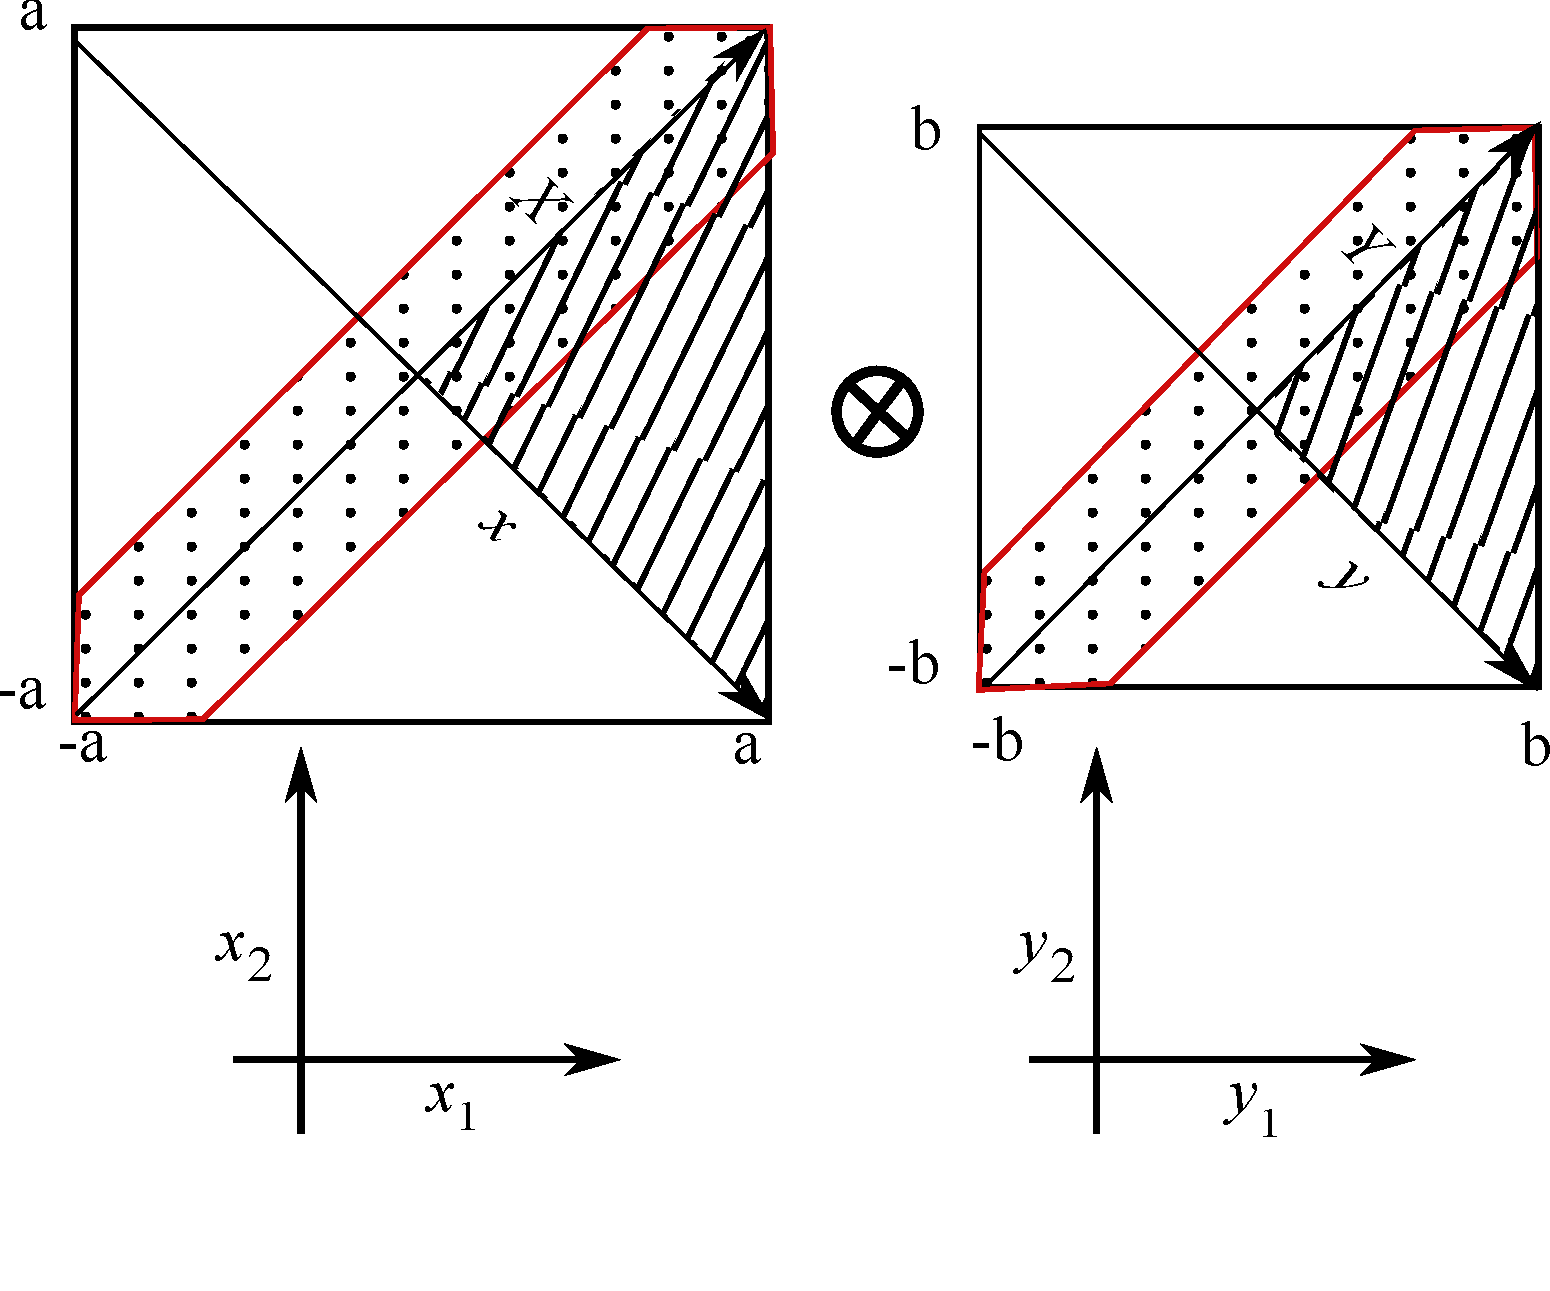
\includegraphics[width=0.80\textwidth]{diagramintegra01.pdf}    
    \end{center}
    Un cubo-4d con un cilíndro atravesado diagonalmente adentro.
  \end{frame}
  
  \begin{frame}
    \frametitle{¿y ahora qué?}
    Las fórmulas (feas y Szabo) dependen sólo de la razón entre
    los radios del anillo (y una $D$ como parámetro). \\
    ¿Cuáles radios?
    En el caso de David, Sebastian et Luca, \emph{preservan área}.\\
    Conservan \emph{el espacio disponible para moverse.}    \\
    En 3d o 4d efectivas ``nos sobran'' parámetros. 
  \end{frame}
  

  \begin{frame}
    \frametitle{Necesitamos conocer entonces V y A}
    Busquemos preservar el \emph{volumen libre} y el 
    \emph{área de contacto}. Parámetros ajustables son
    entonces:
    \begin{itemize}
      \item El radio interior efectivo, $\rho$.
      \item La(s) altura(s), $z, Z$.
     \end{itemize}       
     Convención arbitraria, $z/Z=a/b$.
     \begin{equation}
     \rho(V,A), z(V,A), Z(V,A).  
     \end{equation}

   \end{frame}


  
  \begin{frame}
    \frametitle{Tedioso pero posible (a mano)} 
    \begin{center}
      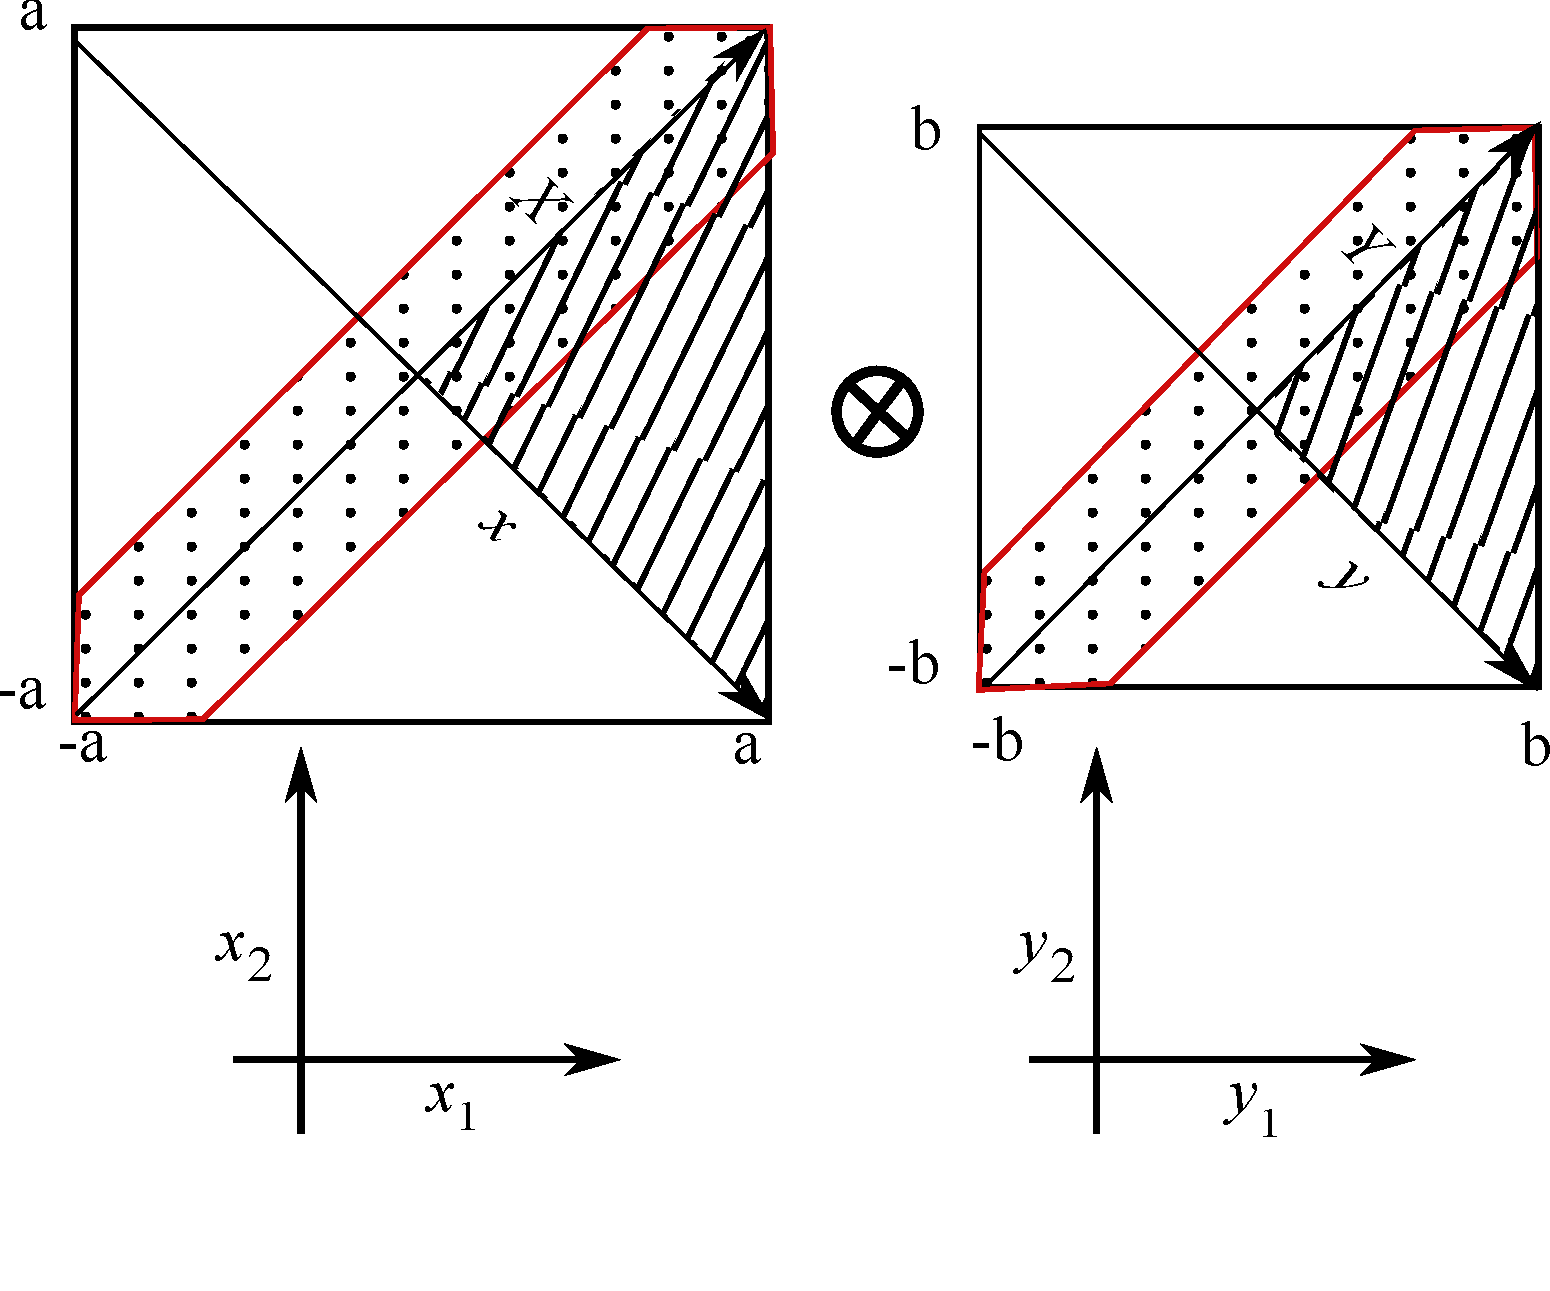
\includegraphics[width=0.70\textwidth]{diagramintegra01.pdf}    
    \end{center}
    \begin{equation}
    V=\iiiint \rd x_1\rd x_2 \rd y_1 \rd y_2
    \indicator{(x_1-x_2)^2+(y_1-y_2)^2\ge (2r)^2}
    \end{equation}
  \end{frame}
   
  \begin{frame}
    \frametitle{``after a little algebra \ldots''}
    \begin{equation}\label{volumeabd}
      V %= 16(I_1 + I_2) =     	
      = 16 a^{2} b^{2}  
      - 16 \pi a b r^{2} 
      + \textstyle \frac{64}{3} (a+b) r^{3}  
      - 8 r^{4},
    \end{equation}
    Rosa Rodriguez, Munakata and Hu (Phys. Rev. E 2002).
    \begin{equation}\label{AreaChoque}
      A  =  16\sqrt{2}\pi a b r -32\sqrt{2} (a+b)r^2 +16 \sqrt{2}r^3 
    \end{equation}
    Usando $V_{int}=\pi R^2 z Z$, $A_{int}=2\pi R zZ$, $z/Z=a/b$:
    \begin{equation}
      R=\frac{2V_{int}}{A_{int}}, \quad  Z^2=\frac{A_{int}^2}{4\pi V_{int} \frac{a}{b}}
    \end{equation}
    Nos quedan unas espantosas expresiones, pero manejables.
  \end{frame}

   
  \begin{frame}
    \frametitle{``after a little algebra \ldots''}
    Ambos ``Cilindros'' tienen las mismas alturas.
    \begin{equation}\label{volumeabd}
      R_{ext}^2=\frac{4 V_{int} V_{cubo}}{A_{int}^2}
    \end{equation}
    \begin{equation}
      \rho=\frac{R}{R_{ext}}=\sqrt{\frac{V_{int}}{V_{cubo}}}
    \end{equation}
    La fórmula de Szabo sólo depende de la raiz del Volumen
    interior (como función de $r$ ) y de constantes.
  \end{frame}
  
  
  \begin{frame}
    \frametitle{La fórmula de Szabo}
    Caso simplificado, $a=b=0.5$, contagio o absorción instantanea:
    \begin{equation}
      \langle \tau  \rangle D /R_{ext}^2=
      (\rho^2-3)/8-\frac{\ln(\rho)}{2(1-\rho^2)}
    \end{equation}
    \begin{center}
      \includegraphics[width=0.65\textwidth]{SzaboTeorica01.pdf}    
    \end{center}
    \end{frame}
  
  
  \begin{frame}
    \frametitle{Numérica}
    Caso simplificado, $a=b=0.5$, contagio o absorción instantanea:
 
    \begin{center}
      \includegraphics[width=0.65\textwidth]{NumericalKarelvsDavid01.pdf}    
    \end{center}
  \end{frame}

  
  
  \begin{frame}
    \frametitle{Numérica}
    Caso simplificado, $a=b=0.5$, contagio o absorción instantanea:
 
    \begin{center}
      \includegraphics[width=0.65\textwidth]{ExperimentoLogSzaboDavidKarel01.pdf}    
    \end{center}
  \end{frame}
  

\end{document}